\label{sec:Res}
\section*{Results}

\subsection*{Constant environment and density-dependence}

We used the previously developed model in \citetext{Sandell et al. 2014, master's thesis} and simulated (see~\autoref{fig:dd}) a tree population for 150 years in a constant environment, with and without density-dependence on $s_0$, assess the effects of a more realistic demography.

As expected, density-dependence allow regulating the population (\autoref{fig:dd} right panel), as the number of mature and immature individuals seem to converge respectively to $18000$ and $10000$ individuals, while without density-dependence the population is exponentially growing.

Looking at the phenotype, we started from exactly the same starting point $z=116$ for phenotypic and genotypic values. Without density-dependence, the population quickly converge to the equilibrium phenotype ($\overline{z_{weak}}$ given by the approximation in~\autoref{eq:zweak}), $\overline{z_{weak}} = 116$ in this case. With density-dependence the equilibrium is shifted towards the survival optimum $\theta_s$ ($\overline{z_{weak, dd}} = 121.8$, $\theta_s = 130$ while $\theta_f = 100$).

The lower seed survival $s_0$ decreases $\gamma_f$~\eqref{eq:gammaf} changing the weights in~\eqref{eq:zweak}, making it more interesting to favor the survival of already established immature trees than the production of many propagules with very little survival prospect.

Within the density-dependent model the mean immature phenotype $\overline{z_I}$ converge quicker than the mean mature phenotype $\overline{z_M}$ to the equilibrium. It is because of stage-structured nature of our model, the mature stage is a combination of individuals that lived for around 40 generations (given our life-cycle), it buffers adaptation. To make $\overline{z_M}$ closer to $\overline{z_{weak}}$, immature individuals with a phenotype closer to $\overline{z_{weak}}$ need to survive long enough to mature and outnumber initial mature individuals with phenotype further from $\overline{z_{weak}}$.

\begin{figure}[ht!]
	\centering
	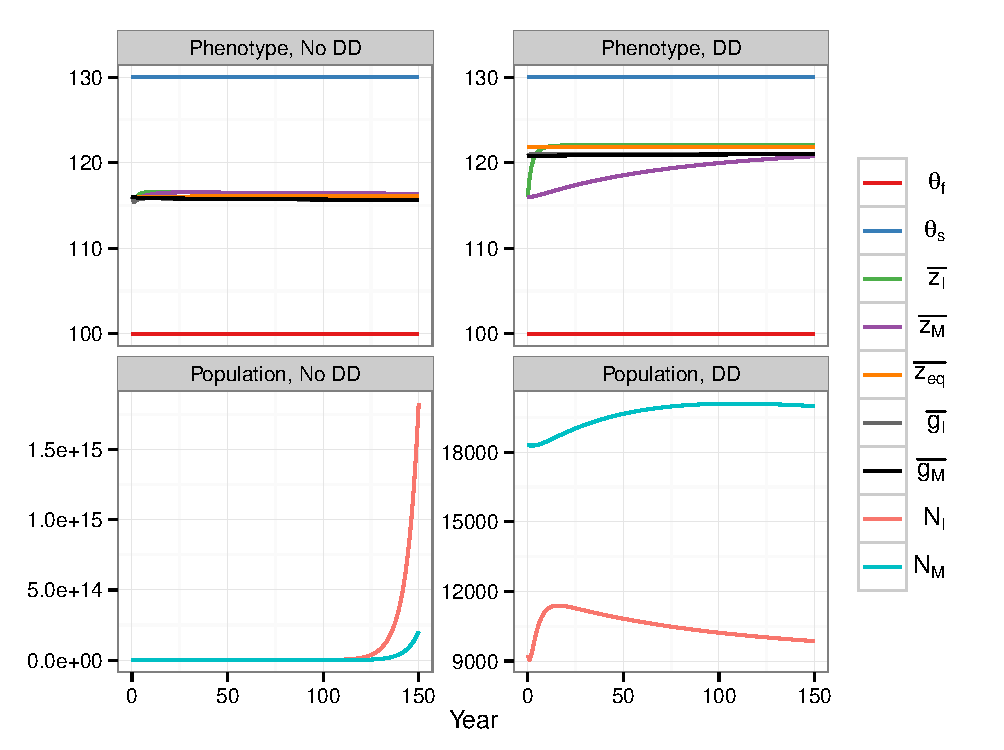
\includegraphics[scale=1]{Figures/DDphenopop.pdf}
	\caption{\textbf{Effect of density-dependence on phenotypes and populations}. \textbf{Left panel}: Phenotype variations in population ($\overline{z_I}, \overline{z_M}$) with their corresponding genotypic values ($\overline{g_I}, \overline{g_M}$) all starting from $z = 116$, and the approximation given by \autoref{eq:zweak}; \textbf{right panel}: demography, number of immature individuals ($N_I$, red), number of mature individuals ($N_M$, blue). Starting from Stable-Stage Distribution (SSD) in constant environment, note the logarithmic scale used.}
	\label{fig:dd}
\end{figure}

\subsection*{Fluctuating optima}

To mimic a more realistic environment we made the optima fluctuate, with various correlations between them. We simulated three populations using the same random seed. We only vary correlations between noises.

Explain in the text correlation of $z_{I}$ with $\theta_{s}(t)$

\begin{figure}[ht!]
	\centering
	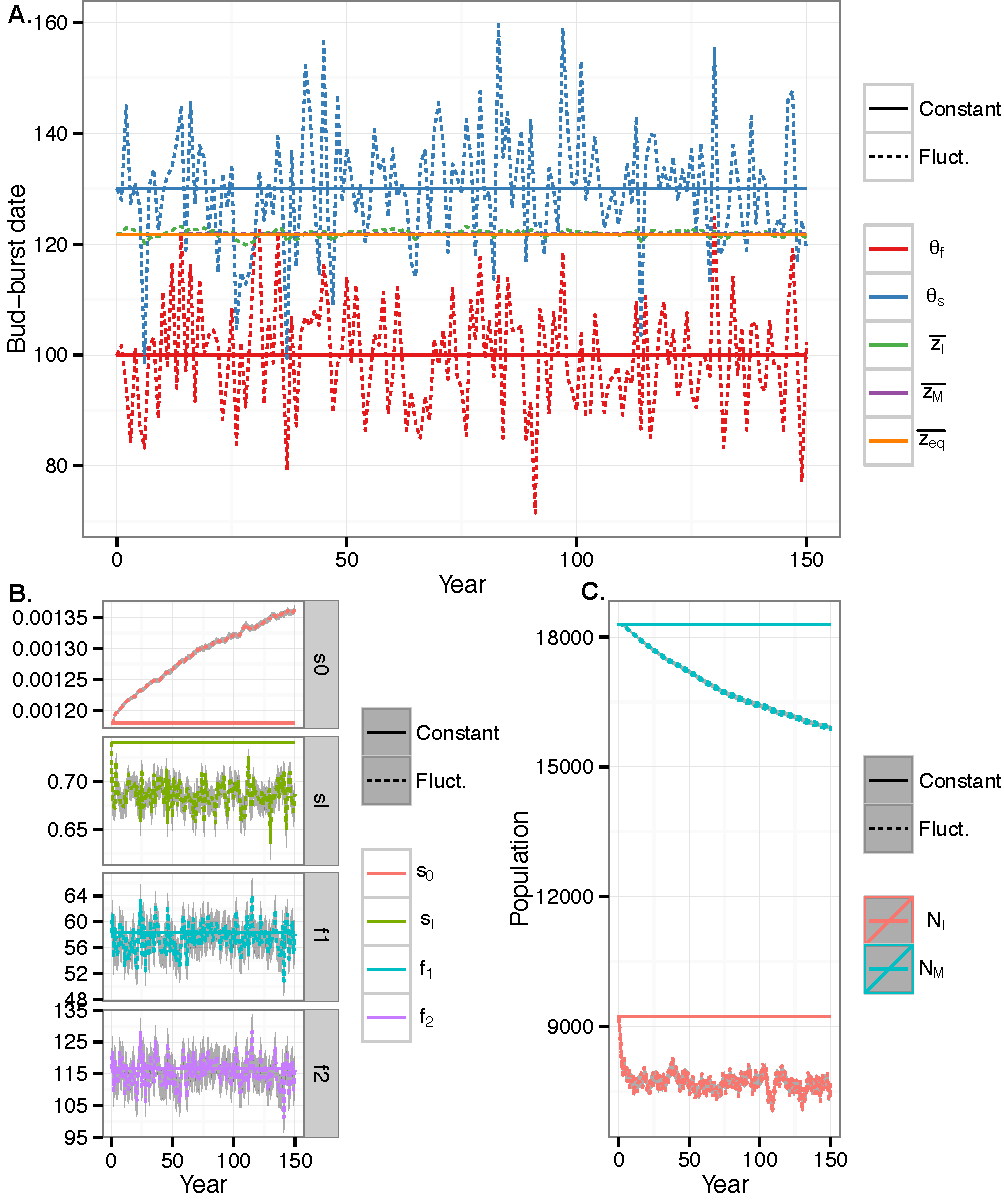
\includegraphics[scale=1]{Figures/PhenoLHTwithCorr.pdf}
	\caption{\textbf{Effect of the correlation of fluctuations on phenotypes and life-history traits}. Correlation coefficient $\rho_{N}$ values of noises are indicated at the the top of each column. Phenotype and approximations are shown in julian days, $\overline{z_\epsilon}$ is the approximation from \autoref{eq:zfluct}. Mean fecundities are in number of seeds produced. The two bottom rows are survival rates, the top one is $\overline{s_I}$ the mean survival of immature individuals, the bottom one is $s_0$ the rate of survival and germination of seeds (see~\nameref{sec:M&M}).}
	\label{fig:corr}
\end{figure}

\subsection*{Trend in the environment}

\begin{figure}[ht!]
	\centering
	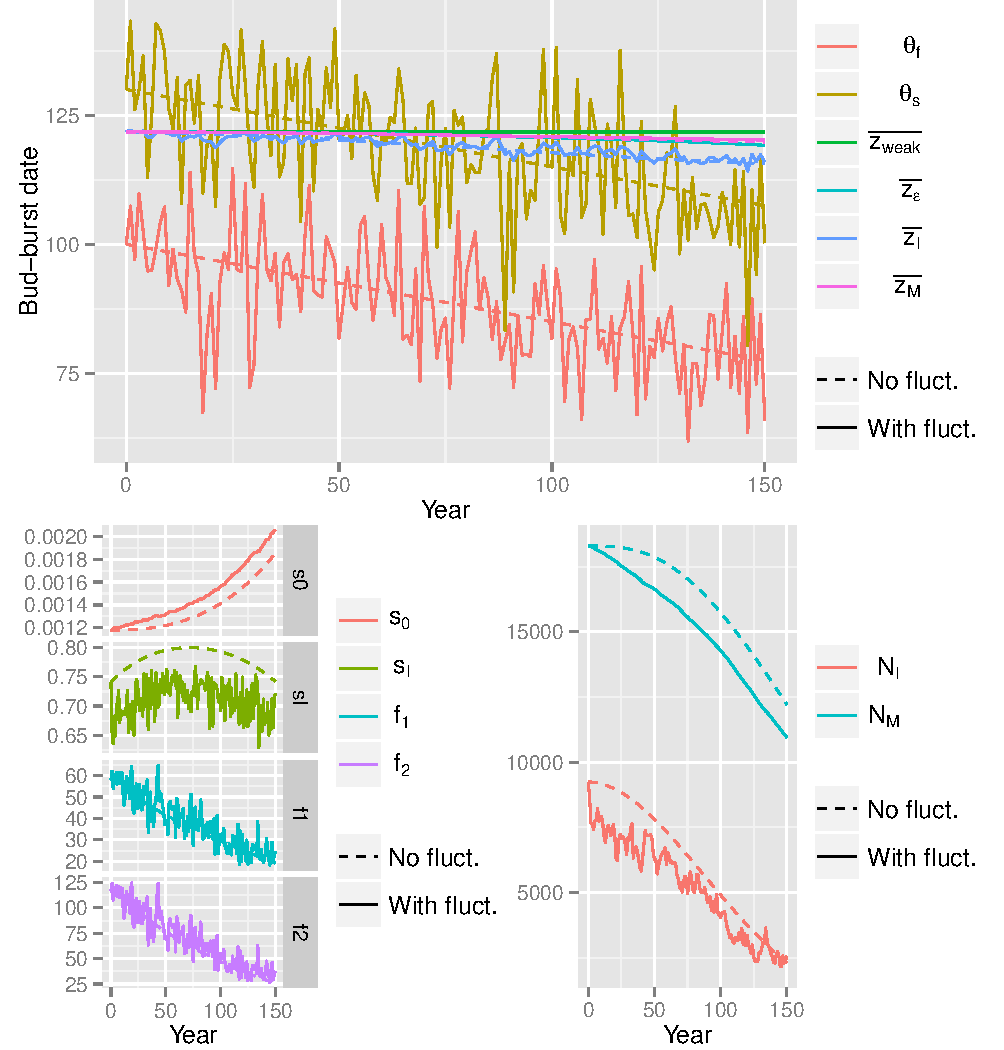
\includegraphics[scale=1]{Figures/Trend.pdf}
	\caption{\textbf{Mixed influences of trend and fluctuations on the population}. \textbf{Top panel}: Phenotype evolution with and without fluctuations, results from a single simulation; \textbf{Bottom panel:} (\textbf{Left}) Life-History Traits evolution depending on fluctuations, survival are rates while fecundities are expressed in produced seeds; (\textbf{Right}) demography. \textbf{With fluct.}: fluctuating optima with a linear trend, \textbf{No fluct.} linearly decreasing optima. Results shown with fluctuations were averaged over 15 independent simulations for demography and life-history traits.}
	\label{fig:trend}
\end{figure}

We implemented a decreasing trend in $\theta_f$ with fluctuations (\autoref{fig:trend}) to mimic climate change. We averaged 15 simulations with fluctuations to understand better the effect of fluctuations.

From~\autoref{fig:trend}, as observed in an environment without a decreasing trend, fluctuations make $\overline{z_I}$ fluctuate, while $\overline{z_M}$ not. It is due to the stage-structure of population, indeed the mature class is a buffers variation because it integrates selection over a very long period; while the immature class have new individuals sensitive to current environment each year.

Looking at life-history traits, $s_I$ has an interesting behavior, it first increases, reaches a maximum, than decreases. The decreasing trend in optima variation causes at first the mean population phenotype to move closer to $\theta_s$, thus maximizing $s_I$ values when it crosses $\theta_s$ line, as soon as it moves beyond $s_I$ starts to decrease again. The fluctuations seem to decrease $s_I$ (mean difference of 0.5), it may be a cost associated with the variance of optimum fluctuations, the optimum is often under the mean population value.

The fluctuations do not seem to affect fecundity differently from the same environment, $f_1$ and $f_2$ decrease because the mean population phenotype go further away from $\theta_f$. Note that they follow exactly the same evolution as the only difference between them is the fecundity value at the optimum date (see \autoref{tab:params}).

Seed germination and survival $s_0$ is increased by fluctuations, via an indirect mechanism: fluctuations decrease immature survival $s_I$, thus decreasing the immature population $N_I$ and so the mature population $N_M$; this population decrease also decrease competition and density, increasing $s_0$ as it is density-dependent (see~\autoref{eq:ddfunc}).

As expected, the decreasing trend in $\theta_f$ creates a lag between the optima and the mean population values, because adaptation is slower than the rate of change. However, the population can still survive with such a rate if the difference between the optima and the means become constant. On a very long scale (~2500 years) it is what happens in this case, the population maintain by changing its phenotype fast enough to track the optima variation (data not shown).

\subsection*{Estimation of the fluctuations}

\begin{figure}[ht!]
	\centering
	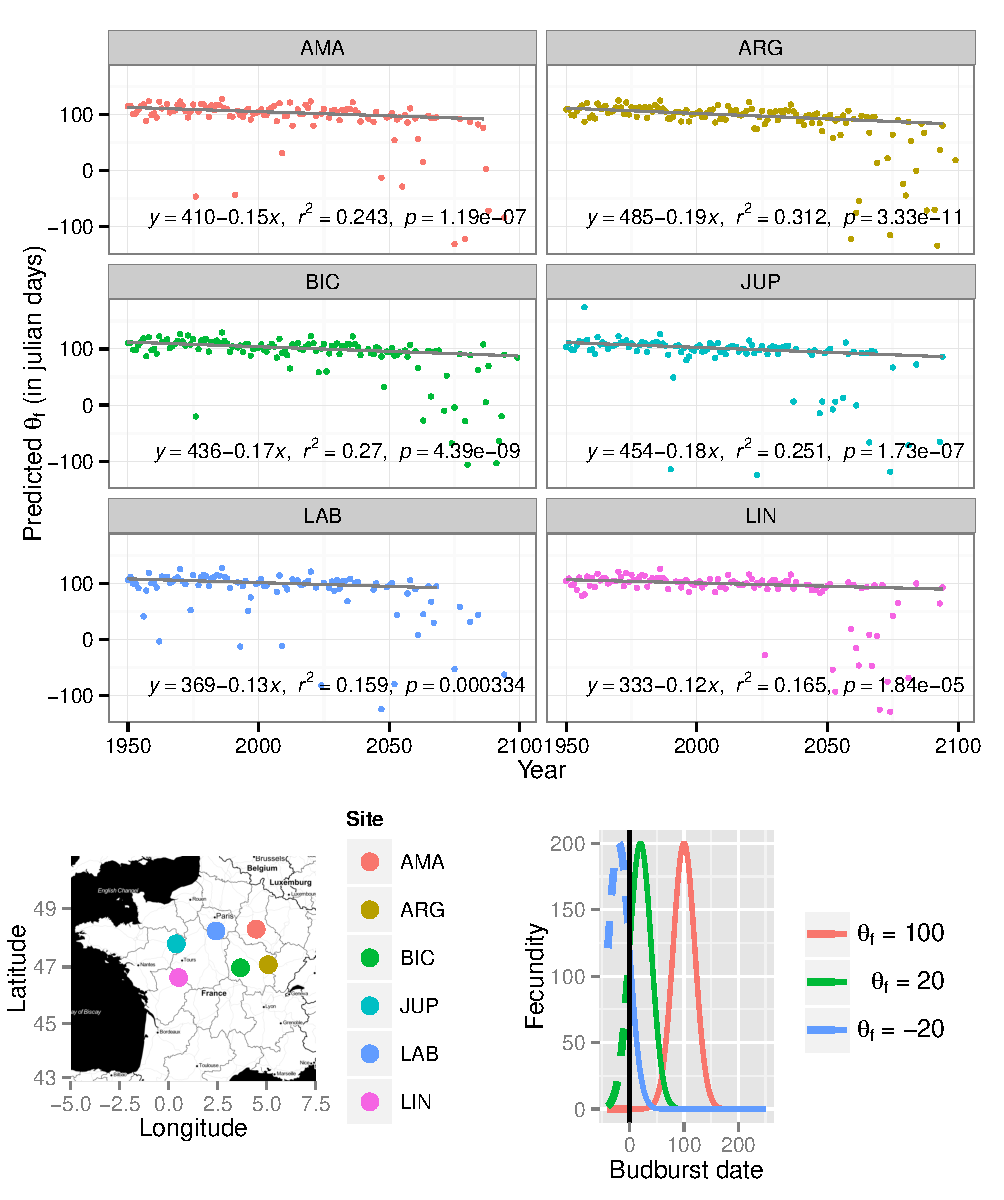
\includegraphics[scale=1]{Figures/optsmaps.pdf}
	\caption{\textbf{$\theta_{f}$ estimations from PHENOFIT data}. Top 3 rows: estimations of $\theta_f$ for each study site see \nameref{sec:M&M} for details. Bottom left panel: map of the study sites. Bottom right panel: Theoretical fecundity functions with parameters from~\autoref{tab:params} with values of $\theta_f$ equals to $100$, $20$ and $-20$, solid lines indicate achievable phenotype, dashed lines show theoretical curves but unreachable phenotypes.}
	\label{fig:thetaf}
\end{figure}

From 6 localities (map \autoref{fig:thetaf} bottom left) of \textsc{PHENOFIT} data, we computed $\theta_f$ values at these locations (top 3 rows of \autoref{fig:thetaf}). For the 6 sites, predicted $\theta_f$ decrease with time, it is more precocious as time passes. This observation matches the advance of phenology observed in the literature because of climate change.

Over the general trend, we observe a small amplitude variation around 20 days, corresponding to year to year change in $\theta_f$ and some dramatic decreases in its values, sometimes reaching negative values (For example at BIC site in 1976). The frequency of these events increase with time as they become \"normal\" after 2050 for all sites. Note that those event are biased towards the decrease of $\theta_f$, as there is no equivalent dramatic increases.

The negative values of $\theta_f$ computed in \autoref{fig:thetaf}, may seem striking as there is no such thing as a negative bud-burst date! However, as bottom right panel of \autoref{fig:thetaf} shows, we can have negative value of $\theta_f$ and still have achievable phenotypes. And if $\theta_f$ is very negative for a given year (less than -100 in 2048 for LAB), it means that will be no reproduction this year.

We excluded those extreme events to estimate the trend in the variation of $\theta_f$ (see~\nameref{sec:M&M}). Using linear regression on $\theta_f$ with time, we found a rate of \SI{-0.15}{\day\per\year}, with normal residuals having a variance of \SI{93.1}{\day\squared} (data not shown, $R^2=0.2435$, $p=1.185\text{\sc{e}-}7$, $F=32.5$ with $101$ d.f.).

We investigated to know if there was a break between years modeled from real data by \textsc{PHENOFIT} (before 2001) and years modeled using climate models with climate change included (from 2001). We performed the same regression as above, without taking apart the extreme values, for all sites, splitting the data before 2001 and from 2001. Taking all years, for each site.